\documentclass[fleqn]{jbook}
\usepackage{physpub}
\usepackage{txfonts}
\begin{document}

\begin{question}{教育 物理}{}


\begin{subquestions}
\SubQuestion
\begin{subsubquestions}
\SubSubQuestion
単位ベクトル$\vec{n}$を軸として角速度$\omega$で回転している座標系の直交
底ベクトルを$\vec{i},\vec{j},\vec{k}$とするとき,ベクトル
\[ \vec{A}=A_x\vec{i}+A_y\vec{j}+A_z\vec{k} \]
の時間変化が
\[\frac{d\vec{A}}{dt}=\frac{dA_x}{dt}\vec{i}+\frac{dA_y}{dt}\vec{j}
+\frac{dA_z}{dt}\vec{k}+\vec{\omega}\times \vec{A} \, ,\, \vec{\omega}
=\omega\vec{n} \]
となることを用いて,一定の角速度$\omega$で回転する座標系における Newton の運動方程式を導き,遠心力とコリオリの力を求めよ。
\SubSubQuestion 
バケツの水を鉛直線のまわりに一定の角速度$\omega$で回転させるとき,水面は遠心力によって放物線となることを示せ。ただし重力加速度を$g$とせよ。 
\SubSubQuestion
 赤道上で,高さ$h$の所から初速ゼロで地面に落下する質点はコリオリの力でど
れだけずれるか。$h=490$mのときのずれの大きさはどれ程か。簡単のため空気
の抵抗は無視できるものとする。
\SubSubQuestion
 A君は{\bf{(iii)}}の問題をコリオリの力を使わないで次のように考えた。地球の半径を
$R$,自転の角速度を$\omega$とすると,慣性系で見た時$h$上空の質点の水平速度は
$(R+h)\omega$,地面の水平速度は$R\omega$だから,結局高さ$h$の点から水平初速度
$h\omega$で発射された質点が放物線を描いて地上に到達するまでの水平距離に等しい
と考えた。その距離を求めよ。しかしこの距離はコリオリの力を用いた{\bf(iii)}の結果と一
致しない。その理由を考察せよ。
\end{subsubquestions}





\SubQuestion
半径$a$の金属円板2枚を間隔$d$で平行に向かい合わせて平行板コンデンサーを作り,
上下の極板にそれぞれ$\pm Q$の電荷を帯電させた。$d\ll a$とし,
円板の縁の電場の乱れは無視できるものとする。

\begin{subsubquestions}
\SubSubQuestion
平行板コンデンサーの静電容量$C$を求め,極板間の電場のエネルギーが
$Q^2/(2C)$に等しいことを示せ。


時刻$t=0$で,両極板間の中心を電気抵抗$R$のまっすぐな針金(半径は$a$に比べ
て十分小さい)で,図1のようにつないだ。$R$は十分大きく,極板間の電荷分布は
常に一様で,自己インダクタンスの効果は無視できるものとする。また,
中心を通る針金からの距離を$r$とする。

\parbox[t]{100mm}{
\SubSubQuestion
 時刻$t$における極板の電荷$q(t)$及び針金を流れる電流$I(t)$を求めよ。
(答えは$C$を含む形で表せ)

\SubSubQuestion
 時刻$t$で極板を流れる電流密度を$r$の関数として求めよ。また,
変位電流はどうなるか。(答えは$I(t)$を含む形で表せ)

\SubSubQuestion
 時刻$t$で極板の間に生じる磁場の極板に平行な成分を$r$の関数として求めよ。
また,コンデンサーの外側ではどうなるか,極板を流れる電流と関係づけて述べよ。

\SubSubQuestion
 電磁場のエネルギーの流れを求め,針金に吸い込まれていくエネルギーと
ジュール熱を比較せよ。
}\parbox[t]{60mm}{
\begin{center}
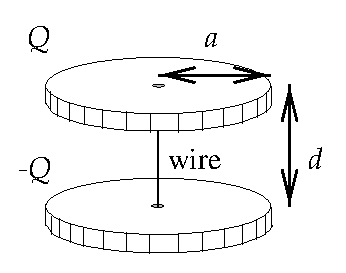
\includegraphics[clip,height=40mm,width=50mm]{1992phys-1.eps}
\end{center}
}
\end{subsubquestions}

\SubQuestion
1モルの理想気体に対して,体積$V$と圧力$p$の平面上で,図2のような状態変化を
考える。$1\rightarrow2,2\rightarrow3,3\rightarrow1$は,それぞれ,準静的等温過
程,準静的等圧過程,準静的等積過程であるとして次の問に答えよ。

\parbox[t]{110mm}{
\begin{subsubquestions}

\SubSubQuestion
 $1\rightarrow2$に対するエントロピー変化$\Delta S_{12}$はいくらか.体積
$V_1,V_2$及び気体定数$R$を用いて表せ。

\SubSubQuestion
 1から2へ断熱的自由膨張で移ったとするとき,$\int d'Q/T$を求めよ。但
し,$T$は温度,$Q$は熱量である。この結果を前問の$\Delta S_{12}$と比較
することにより何がわかるかを説明せよ。

\SubSubQuestion
 1から始まる準静的断熱過程により,2と3を結ぶ直線上の4に到達したと
する。準静的断熱過程では$TV^{\gamma-1}$が一定であることを示せ。但し,
$\gamma$は定圧モル比熱と定積モル比熱の比である。これを用いて,$V_4$の
表式を$V_1,p_1,p_2$の関数として求めよ。

\SubSubQuestion
 $1\rightarrow4,4\rightarrow3,3\rightarrow1$に対するエントロピー変化をそ
れぞれ計算せよ。循環過程$1\rightarrow4\rightarrow3\rightarrow1$における
エントロピー変化はいくらになるはずか。これを用いて,前問と同じ$V_4$の表式を求
めよ。
\end{subsubquestions}}
\parbox[t]{50mm}{
\begin{center}
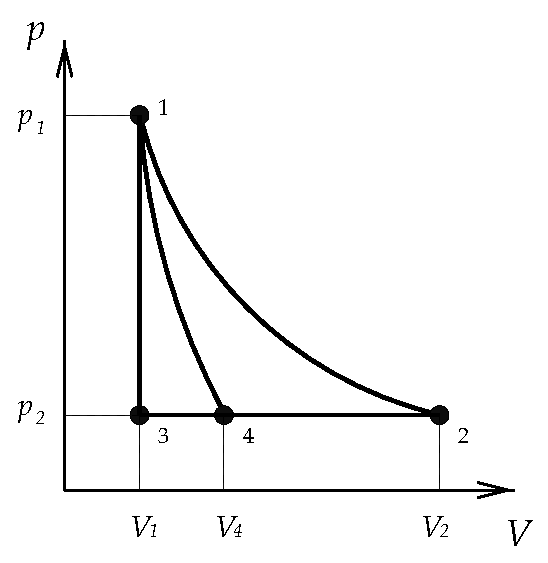
\includegraphics[clip,height=53mm,width=45mm]{1992phys-2.eps}
\end{center}
}

\end{subquestions}
\end{question}
\begin{answer}{教育 物理}{}
\begin{subanswers}

\SubAnswer
\begin{subsubanswers}
%定義がなされている。ぶつかりに注意
\newcommand{\td}[1]{\frac{d #1}{dt}}
\newcommand{\dv}[1]{\td{\vec{#1}}}

\SubSubAnswer
$ \vec{A}= A_x \vec{i} + A_y \vec{j} + A_z \vec{k} $
を時間微分すると
\[ \dv{A} = \td{A_x}\vec{i} + \td{A_y}\vec{j} + \td{A_z}\vec{k} + A_x\dv{i} + A_y\dv{j} + A_z\dv{k} \]
これを与えられた式
\[ \dv{A}= \td{A_x}\vec{i}+ \td{A_y}\vec{j} + \td{A_z}\vec{k} + \vec{\omega} \times \vec{A} \]
と比べて
\begin{eqnarray}
A_x \dv{i} + A_y \dv{j} + A_z \dv{k} = \vec{\omega} \times \vec{A} \eqname{5p1-1}
\end{eqnarray}
を得る。ここで $ \vec{r}=x\vec{i} + y\vec{j} + z\vec{k} $ に対して
\begin{eqnarray}
\dot{\vec{r}} = \dot{x}\vec{i}+ \dot{y}\vec{j}
 +\dot{z}\vec{k} + \vec{\omega}\times\vec{r} \eqname{5p1-2}
\end{eqnarray}
さらに時間微分を行って
\[ \ddot{\vec{r}} = \ddot{x}\vec{i} + \ddot{y}\vec{j} + \ddot{z}\vec{k} + \dot{x}\dv{i} + \dot{y}\dv{j} + \dot{z}\dv{k} + \vec{\omega}\times\dot{\vec{r}} \]
ただし $\vec{n}$ は定ベクトルなので $\dot{\vec{\omega}} = \omega\dot{\vec{n}} = 0 $ を用いた。 \eqhref{5p1-1},\eqhref{5p1-2} を代入して
\[ \ddot{\vec{r}} = \vec{a} + 2\vec{\omega}\times{\vec{v}} + \vec{\omega}\times{\left(\vec{\omega}\times\vec{r}\right)} \]
ただし $\vec{a} \equiv \ddot{x}\vec{i} + \ddot{y}\vec{j} + \ddot{z}\vec{k}$ 、 
$\vec{v}\equiv\dot{x}\vec{i}+\dot{y}\vec{j}+\dot{z}\vec{k} $ はそれぞれ回転座標系における加速度および速度にあたる。

外力 $\vec{F}$ は $m\ddot{\vec{r}}$ に等しいから
\[ m\vec{a} = \vec{F} - 2m\vec{\omega}\times\vec{v} - m\vec{\omega}\times\left(\vec{\omega}\times\vec{r}\right) \]
第 $2$ 項がコリオリ力、第 $3$ 項が遠心力に対応する。

\SubSubAnswer
\parbox[t]{100mm}{
水面が安定する条件を考える。水面付近の水にその水面と垂直でない成分を持つ力が働くと、そこの水はその方向に動いて
しまうと考えられる。よって水面が安定するにはその水面に対し垂直な力のみが働く時になる。そして、これが圧力 $\vec{P}$ に
よって支えられている。図のように水面の水の位置ベクトルを回転の中心軸から $\vec{\omega}$ に垂直にとる。また水面の高さを $f(x)$ であらわすと 
\[ 0 = -mg \frac{\vec{\omega}}{\omega} + \vec{P} + m\vec{\omega}^2 \vec{r} \]
$\vec{\omega}/{\omega}$ と $\vec{r}/r $ を成分で表すと
}\parbox[t]{60mm}{
\begin{center}
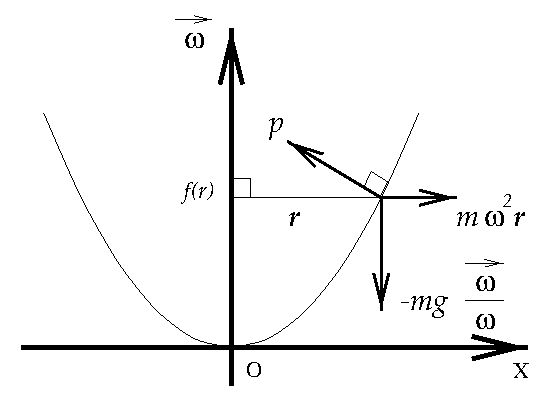
\includegraphics[clip,height=40mm,width=50mm]{1992phys-3.eps}
\end{center}
}

\begin{eqnarray}
0 & = & -mg + P \frac{1}{\sqrt{1+{f'\left(x\right)}^2}} \\
0 &=& {} - P \frac{f'\left(r\right)}
{\sqrt{1+{f'\left(r\right)}^2}} + m \omega^{2} r 
\end{eqnarray} 
 $P$ を消去して 
\[ f'\left(r\right) = \frac{{\omega}^2}{g}r \]
積分して 
\[ f\left(r\right) = \frac{{\omega}^2}{2g}r^{2} + C_{0} \]
但し $C_{0} $ は定数である。

以上より水面は放物線になることがわかる。

\SubSubAnswer
回転座標系を円柱座標で表す。
\[
\vec{e} _{r} = \left(\cos \theta , \sin \theta ,0 \right) \quad 
\vec{e} _{\theta} = \left( - \sin \theta , \cos \theta , 0 \right) \quad
\vec{e} _{z} =  \left( 0,0,1\right) 
\]
であるから

\parbox[t]{100mm}{
\[ \dot{\vec{e}}_{r} = \vec{e}_{\theta} \dot{\theta} ,\quad
\dot{\vec{e}}_{\theta} = - \vec{e}_{r} \dot{\theta} ,\quad  \dot{\vec{e}}_{z} =\vec{0} \]
となる。よって $\vec{r} = r\vec{e}_r $ を時間微分すると
\[\dot{\vec{r}} = \dot{r} \vec{e}_{r} + r\dot{\theta}\vec{e}_{\theta}\]
\[\ddot{\vec{r}}= \left(\ddot{\vec{r}}- r\dot{\theta}^2 \right)\vec{e}_{r} + \left(2\dot{r}\dot{\theta} + r \ddot{\theta} \right) \vec{e}_{\theta}
\]

図のように座標系をとると
\[ m \vec{a} = -mg \vec{e}_{r} - 2m \vec{\omega}\times\vec{v} + m{\omega}^{2}r\vec{e}_r \]
$ \vec{a} \Rightarrow \ddot{\vec{r}}$ 、 $\vec{v} \Rightarrow \dot{\vec{r}}$ と
置き換えて $\vec{e}_r$ 成分と $\vec{e}_{\theta} $ 成分に分けると
\[ \ddot{r} - r\dot{\theta}^2 = -g + \omega^{2} r + 2\omega r \dot{\theta} \]
\[ 2\dot{r}\dot{\theta} + r \ddot{\theta} = -2\omega \dot{r} \]
}\parbox[t]{60mm}{
\begin{center}
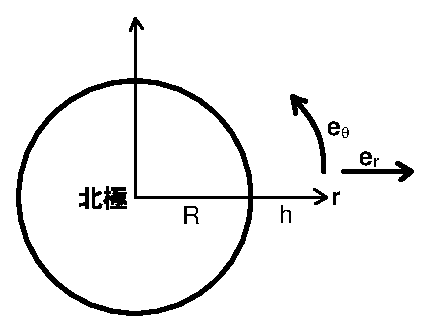
\includegraphics[clip,height=40mm,width=55mm]{1992phys-3-1.eps}
\end{center}
}

ただしコリオリ力$F$は 
\[
F=-2m \vec{\omega} \times \vec{v}= -2m\omega \vec{e}_z \times \left(\dot{r} \vec{e}_r + r\dot{\theta}\vec{e}_{\theta} \right) = -2m\omega \left( \dot{r}\vec{e}_{\theta} - r\dot{\theta}\vec{e}_{r} \right) 
\]
と計算した。 $\vec{e}_{\theta} $ 成分の式は
\[
r\td{\dot{\theta}} = -2 \td{r}\left(\dot{\theta} + \omega \right) \quad 
\leftrightarrow   \td{\ln\left(\dot{\theta} + \omega \right)} = -2
\td{\ln r} \quad
\leftrightarrow   \left(\dot{\theta} + \omega \right) = \frac{C}{r^{2}} 
\]
と積分ができ、初期条件 $ \dot{\theta} = 0$ , $ r = R + h$ を代入して
\begin{eqnarray}
\dot{\theta} = \omega \left(\frac{\left(R+h\right)^2}{r^2} - 1 \right)  \eqname{equation1-3-1}
\end{eqnarray}
ここで $r$ は $R+h \sim R $ の値をとり $R \gg h $ を考えると $\dot{\theta}$ は
$\omega$ ぐらいかそれよりも小さい値をとる。よって運動方程式の $\vec{e}_r$
成分は
\[\ddot{r} = -g\left( 1 + {\cal O}\left( \frac{\omega ^{2} R}{g} \right)\right) \]
となる。実際に地球の自転、半径を入れて見ると
\[ \frac{\omega ^2 R}{g} = \left(\frac{2\pi }{24 \times 60 \times 60}\right)^2 \frac{6.4 \times 10^{6} }{9.8} \sim 0.003 \]
この項は微小になり無視できる。 $\dot{r} (t=0) =0 $ , $r(t=0) = R+h$ であるから
\[ r = \left(R+h\right) - \frac{gt^2}{2} \]
これを式\eqhref{equation1-3-1}に代入して
\[
\dot{\theta} = \omega  \left\{ \frac{\left(R+h\right)^2}{ \left( \left(R+h\right)-gt^2/2  \right) ^2} -1 \right\} 
= \omega \left\{ {\frac{1}{ \left( 1 - gt^2/2\left(R+h\right)  \right)^2} -1 } \right\} 
\simeq \omega \left( 1 + \frac{gt^2}{R+h} -1 \right) 
= \frac{\omega g t^2 }{R+h} 
\]
これを積分して
\[ \theta = \frac{\omega g t^3}{3\left(R+h\right)} \]
質点が落下する $\left( r=R+h \ \rightarrow \ r=R\right)$ のに要する時間は
${\displaystyle{ r = \left(R+h\right) - \frac{gt^2}{2} }}$
より
${\displaystyle{ t = \sqrt{\frac{2h}{g}} }}$
この間 $\theta $ は $\theta = 0$ から
\[ \theta = \frac{\omega g}{3\left(R+h\right)} \Bigl(\sqrt{\frac{2h}{g}}\Bigl)^3 \]
だけずれる。これは地表面では $( h/R \ll 1)$
\[ \frac{\omega g}{3}\Bigl(\sqrt{\frac{2h}{g}}\Bigl)^3 \frac{R}{R+h} \simeq \frac{\omega g}{3}\Bigl(\sqrt{\frac{2h}{g}}\Bigl)^3 \]
$h=490{\rm m}$ の場合
\[ \frac{2\pi}{24 \times 60 \times 60} \frac{9.8}{3}\Bigl(\sqrt{\frac{2\times490}{9.8}}\Bigl)^3 = 24{\rm cm} \]

\SubSubAnswer

地上に達するまでには
${\displaystyle{ t = \sqrt{\frac{2h}{g}} }}$
かかる。初速度が $h\omega$ ならばこの間に
${\displaystyle{ h\omega t = h\omega \sqrt{\frac{2h}{g}} }}$だけ
進む。これは明らかに{\bf{(iii)}} の答え
\[ \frac{\omega g}{3}\Bigl( \sqrt{\frac{2h}{g}}\Bigl)^3 = \frac{2}{3}h\omega \sqrt{\frac{2h}{g}} \] 
と異なる。この考察に地球の回転が質点が発射された瞬間においてのみ加味されている
からである。つまり質点の相対速度は高さ $x{(\rm m)} $ の時 $ x \omega$ である
のだからずれる距離は$\displaystyle{\int_{x=h}^{x=0} x\omega dt}$
で与えられる。これに$\displaystyle{ x= h -\frac{gt^2}{2}}$
を代入すれば
\[
\int_{t=0}^{t=\sqrt{2h/g}} \left(h- \frac{gt^2}{2}\right)\omega dt
= \omega   [ ht - \frac{gt^3}{6}  ] _{t=0}^{t=\sqrt{2h/g}}
=\frac{2}{3} \omega h \sqrt{\frac{2h}{g}}
\]
と答えは一致する。
\end{subsubanswers}

\SubAnswer
\begin{subsubanswers}
\SubSubAnswer
極板間の電場と電位差は、ガウスの法則より
\[
E = \frac{Q}{\varepsilon _0 \pi a^2} ,V = \frac{Qd}{\varepsilon _0 \pi a^2}
\]
よって、$Q=CV$より
\[
C = \varepsilon _0 \frac{\pi a^2}{d}
\]
よって、電磁場のエネルギーは
\[
\frac{1}{2}\varepsilon _0E^2\pi a^2d = \frac{Q^2d}{2\varepsilon _0 \pi a^2}
= \frac{Q^2}{2C}
\]

\SubSubAnswer
極板間には電位差 $ V = Q/C $ があるのでこれによって針金には電流が流れる。
よって
\[ I(t)= \frac{V}{R} = \frac{q(t)}{RC} \]
$I(t) $ は極板上の電荷が減少して針金に流れ込む事によって流れるのだから
$ I(t)= -dq(t) / dt $ 。よって
\begin{eqnarray*}
- \frac{dq}{dt} & =& \frac{q(t)}{RC} \Rightarrow q(t) = q(0)\exp (-t/RC) \\
 & \Leftrightarrow & I(t)=\frac{q(0)}{RC}\exp \left(-t/RC\right)
\end{eqnarray*}

\SubSubAnswer
\parbox[t]{100mm}{
極板上の電荷は一様に減って中心の針金に流れるのであるから、その流れは
中心に向かっていて、中心に対して対称のはずである。そこで半径 $r(<a)$ の
点における弧に対する電流線密度を $\vec{i}(r)$ とする。時間 $dt$ に図の部分から中心に向かう電荷はその定義によ
り $i(r)\cdot r d\theta \cdot dt $ となる。これはその外側の部分から
 $i(r+dr) \cdot (r+dr)d\theta \cdot dt$ だけ、また斜線部から電荷が減少
することによって $-dq(t) / \pi a^{2} \times r d \theta dr $ だけ供給
される。よって

}\parbox[t]{60mm}{
\begin{center}
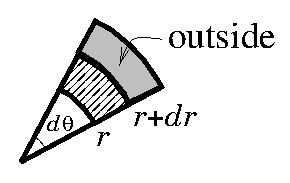
\includegraphics[clip]{1992phys-4-2.eps}
\end{center}
}

\[ i(r)r d\theta dt = i(r+dr) \cdot (r+dr)rd\theta \cdot dt - dq(t)/\pi a^{2} \cdot rd\theta dr \]
$ -dq(t) = I(t)dt $ に注意して

\[
\leftrightarrow \frac{i(r+dr)\cdot (r+dr) - i(r)r}{dr} = -\frac{I(t)r}{\pi a^{2}} 
\leftrightarrow \frac{d}{dr}{i(r)\cdot r} = -\frac{I(t)r}{\pi a^2} 
\leftrightarrow i(r)dr = -\frac{I(t)r^{2}}{2\pi a^{2}} +C 
\]

極板の周辺 $(r=a)$ では電流供給源が無いから $\vec{i}(r=a)=0$ のはず。
\[
i(a)\cdot a = -\frac{I(t)a^2}{2\pi a^2} + C = 0 
\leftrightarrow C = \frac{I(t)}{2\pi} 
\]

これより
\[ i(r) = \frac{I(t)}{2\pi r} \left( 1 - \left(r/a\right)^2  \right) \]

これは境界条件 $i\cdot 2\pi r= I(t) (r \rightarrow 0)$ も満たす。
このことは極板上の電流は全て $r\rightarrow 0 $ でまとまっていて $I(t) $ と
なって針金を流れると言うことをいっている。

変位電流は極板間の電束密度の減少を説明するもので
\[
\frac{\partial D}{\partial t} = i_e 
\leftrightarrow i_e = -\frac{\partial}{\partial t} \left(
\varepsilon _0\frac{V(t)}{d} \right) 
= -\frac{\partial}{\partial t}\varepsilon _{0} \frac{R}{d}I(t) 
= \frac{\varepsilon _{0}}{Cd} I(t) 
= \frac{I(t)}{\pi a^2} 
\]
ただし $C=\varepsilon _0 \pi a^2 / d$ としている。
実際 $\vec{D}$ の減少は $I(t)$ によるもので、この減少が一様におきているならば
電流密度が一様に $I(t)/\pi a^{2}$ と分布していて、これが原因と考えられるので
{\it O.K.}

\SubSubAnswer

\parbox[t]{40mm}{
\begin{center}
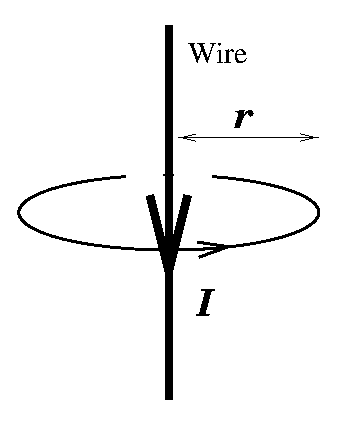
\includegraphics[clip,height=40mm,width=30mm]{1992phys-4.eps}
\end{center}}\parbox[t]{120mm}{
その対称性により磁場の極板に平行な成分は極板との距離によらず円周方向成分
のみを持つ。そこで左の図のような経路に対して
\[ \nabla \times \vec{H} - \frac{\partial \vec{D}}{\partial t} = \vec{i}_{e} \]
を表面積分すると
\[ \int \vec{H}d\vec{s} - \frac{\partial}{\partial t}\int \vec{D}d\vec{s} = \int \vec{i} d\vec{s} \]
\[ \leftrightarrow \begin{cases}
        H(r)2\pi r - \frac{I}{\pi a^{2}} \pi r^{2}= -I &(r\le a) \\
        H(r)2\pi r - \frac{I}{\pi a^{2}} \pi a^{2}= -I &(r > a) \\
        \end{cases}\]
\[ \leftrightarrow \begin{cases}
        H(r)=-\frac{I}{2\pi r} \left(1-\left(r/a\right)^2\right)=-i(r) & (r\le a) \\ 
       H(r)=0 & (r > a) \\
        \end{cases}\]
        }
\parbox[t]{110mm}{
これは右の図の経路を使っても求められる。
この場合、この経路に
よって囲まれた面に垂直な $\vec{D}$ 成分は無いので
\[ \nabla \times \vec{H} = \vec{i}_{e} \]
面に流れ込んで来るのは極板上の電流線密度である。よってこの表面積分は
\begin{itemize}
\item $r \ge a $ の時 
\[ H_{in}\cdot 2\pi r - H_{ex} \cdot 2\pi r = \vec{i} \cdot 2\pi r \]
\[ H_{in}(r) = \vec{i} + H_{ex} (r) \]
\item $r < a $ の時 
\[ H_{in} \cdot 2\pi r = H_{ex} \cdot 2\pi r = 0 \]
\[ H_{in} (r) = H_{ex}(r) \]
\end{itemize}}\parbox[t]{50mm}{
\begin{center}
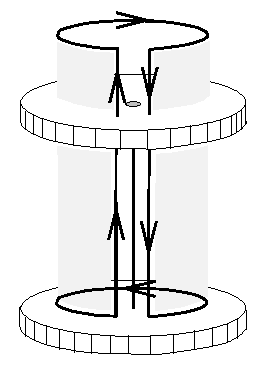
\includegraphics[clip,height=50mm,width=40mm]{1992phys-5.eps}
\end{center}}

\parbox[t]{50mm}{\begin{center}
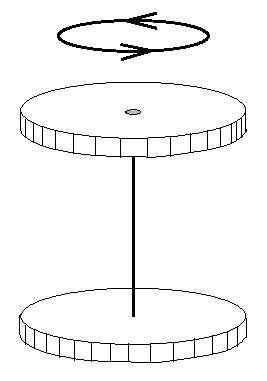
\includegraphics[clip,height=40mm,width=40mm]{1992phys-6.eps}
\end{center}}\parbox[t]{110mm}{
極板の上で表面積分を上の図のように行えば
\[ H_{ex} \cdot 2 \pi r = 0 \leftrightarrow H_{ex} = 0 \]
よって
\[ H_{in} (r) = \begin{cases}
                -i  & (r\le a ) \\
                0   & (r > a )
        \end{cases}\]
と同様の事が導かれる。

コンデンサーの外側で磁場が無いのは前者の解法によれば針金を流れる電流が
作る磁場を電束密度が変化する事により生じる磁場がちょうど打ち消すためである。この電束密度の変化は極板上の電荷が減少するためであり、言葉を変えると、極板
を流れる電流のためと言える。つまり、外側で磁場が無いのは針金の電流が作る
磁場を極板を流れる電流が打ち消すためであると言える。}

\SubSubAnswer
電磁場のエネルギーの流れは Poynting Vector
\[ \vec{S} = \vec{E} \times \vec{H} \]
から求められる。 $\vec{E}$ が極板 $Q$ から極板 $-Q$ 向きへ、 $\vec{H}$ が
極板 $Q$ から見て右周りであるから $\vec{S}$ は針金に向かう。 $\vec{H}$ と
 $\vec{E}$ とは交わっているから
\[
S = \frac{V}{d}\frac{I}{2\pi r} \left( 1 - \left(r/a\right)^2 \right) 
 =  \frac{RI^2}{2\pi rd} \left( 1 - (r/a)^2 \right) 
\]
針金に吸い込まれて行くエネルギーは針金の半径を $\rho \gg a$ として
\[
S_{\rho} \cdot 2\pi \rho d = \frac{RI^2}{2\pi \rho d} \left( 1 - \left(\rho / a
\right)^2 \right) 2 \pi \rho d 
= RI^{2} \ \left(\rho / a \gg 1\right) 
\]
また Joule 熱は  $VI = RI^{2} $となるから、
と一致しており、電磁場のエネルギーが針金で Joule 熱になっていると
いえる。

\end{subsubanswers}

\SubAnswer
\begin{subsubanswers}
理想気体では、
$\displaystyle{dU = C_{V} dT}$
であり、等温過程では
$\displaystyle{
dU = 0
}$
でるから、熱力学第一法則より、
$\displaystyle{
d'Q = p dV
}$

ここで、1モルの理想気体の状態方程式
$\displaystyle{
pV =RT
}$
から、pを消去して整理すると、
\[
\frac{d'Q}{T} = R\frac{dV}{V}
\]
したがって、$1 \rightarrow 2$に対するエントロピーの変化は次のようになる。
\[
\Delta S_{12} =  \int \frac{d'Q}{T}
              = \int_{V_{1}}^{V_{2}}\frac{RdV}{V}
             =   R\ln \frac{V_{2}}{V_{1}}
\]

\SubSubAnswer

断熱膨張過程では、$d'Q=0$であるから、
\[
\int\frac{d'Q}{T} = 0
\]
断熱自由膨張過程が準静的であるとすると、これが$1 \rightarrow 2$
に対するエントロピー変化を与えることになる。
しかし、準静的な変化であれば、過程によらず同じエントロピー変化が
得られるはずである。したがって{\bf{(i)}}との比較から、断熱自由膨張過程が
準静的でないことがわかる。

\SubSubAnswer
準静的断熱過程では$dQ'=0$であるから、熱力学第一法則より
$\displaystyle{
C_{V}dT + pdV = 0
}$が成り立つ。

ここで状態方程式より、
$\displaystyle{
pV =RT
}$から、
$p$を消去して整理すると、
\[
\frac{dV}{T} + \frac{R}{C_{V}}\frac{dV}{V} = 0
\]
両辺積分して整理すると、
$\displaystyle{
TV^{\frac{R}{C_{V}}} = const.
}$
となる。

さて、マイヤーの法則
$\displaystyle{
C_{P} = C_{V} + R
}$
を変形して、
\[
\frac{R}{C_{V}} = \gamma -1
\]
したがって、
$\displaystyle{
TV^{\gamma -1} = const.
}$
。また、状態方程式より$T$を消去すると、
$\displaystyle{
pV^{\gamma}=const.
}$。

これより、
$\displaystyle{
p_{1}V_{1}^{\gamma} = p_{2}V_{4}^{\gamma}
}$
よって、
$\displaystyle{
V_{4} = V_{1} \left( \frac{p_{1}}{p_{2}} \right)^{1/\gamma}
}$

\SubSubAnswer
$1 \rightarrow 4$:\\
断熱過程であることから$dQ'=0$。よって、
$
\Delta S_{12} = 0
$。

$4 \rightarrow 3$:\\
理想気体では$dU = C_{V}dT$であり、$p=p_{2}$の等圧過程であるかことから、
\[
d'Q = C_{V}dT + p_{2}dV
\]
ここで、状態方程式$p_{2}V=RT$の微分から、
$
p_{2}dV = RdT
$
なので、
\[
d'Q = \frac{C_{V}}{R}p_{2}dV + p_{2}dV
\]
マイヤーの関係式を使えば、
\[
d'Q = \frac{C_{P}}{p_{2}}dV
\]
また、状態方程式から$p_{2}$を消去すれば、
\[
d'Q = \frac{C_{P}}{R}\frac{RT}{V}dV
\Longleftrightarrow 
\frac{d'Q}{T} = C_{P}\frac{dV}{V}
\]
よって、この過程におけるエントロピー変化は、
\[
\Delta S_{43} =  \int\frac{d'Q}{T} 
              =  \int_{V_{4}}^{V_{1}}C_{P}\frac{dV}{V}
              =   C_{P}\ln\frac{V_{1}}{V_{4}}
\]
$3 \rightarrow 1$:\\
熱力学第一法則より、
$\displaystyle{
d'Q = C_{V} dT
}$。
状態方程式を微分した式をもちいれば、
\[
dT = \frac{V_{1}}{R}dp = T\frac{dp}{p}
\]
したがって、
\[
d'Q = C_{V}T\frac{dp}{p}
\Longleftrightarrow 
\frac{d'Q}{T} = C_{V}\frac{dp}{p}
\]
よってこの過程におけるエントロピー変化は
\[
\Delta S_{31} =  \int\frac{d'Q}{T}
              =  \int_{p_{2}}^{p_{1}}C_{V}\frac{dp}{p}
              =   C_{V}\ln\frac{p_{1}}{p_{2}}
\]

以上より、循環過程$1 \rightarrow 4 \rightarrow 3\rightarrow 1$
におけるエントロピー変化は、
\[
\Delta S_{14} + \Delta S_{43} + \Delta S_{31}
= C_{P}\ln\frac{V_{1}}{V_{4}} + C_{V}\ln\frac{p_{1}}{p_{2}}
\]

このエントロピー変化は0になるはずなので、
\begin{eqnarray*}
V_4=V_1 \Bigl(\frac{p_1}{p_2}\Bigl)^\frac{C_v}{C_p}
\end{eqnarray*}
\end{subsubanswers}


\end{subanswers}
\end{answer}




\end{document}


